\documentclass{beamer}

\usepackage{color}
\usepackage{framed}
\usepackage{fancyvrb}
% \usepackage{listings}

\usepackage{beamerthemesplit}
\usepackage{graphicx}
\usepackage{verbatim}
\usetheme{Dresden} % Ja, naturlich!


% Any multidimensional value (point, vector, etc.)
\newcommand\Nd[1]{\mathbf{#1}}

% Arrays, Vectors, and Points are all bold, with additional (mostly
% LaTeX) conventions:
\newcommand\A[1]{\Nd{#1}}
% note: "\vec\Nd" does the right thing; "\Nd\vec" doesn't.
\newcommand\V[1]{\vec{\Nd{#1}}}
\newcommand\Pt[1]{\tilde{\Nd{#1}}}

% Normalize (as a function)
\newcommand\normalize[1]{\widehat{#1}}

% Unit-length vectors (with hats)
\newcommand\U[1]{\normalize{\Nd{#1}}}

% Components of unit-length vectors (with hats)
\newcommand\Usub[2]{\normalize{#1}_{#2}}

% Dot product
\newcommand\vdot[2]{({#1} \cdot {#2})}

% Flag forward references
\newcommand\tbd[1]{{\color{red} #1}}

% Rgb (multispectral) values
\newcommand\rgb[1]{\Nd{#1}}

% Matrices
\newcommand\mat[1]{\Nd{#1}}

% Vector magnitude
\newcommand\vmag[1]{\left|#1\right|}

% Absolute value of dot product
\newcommand\absvdot[2]{\left|{#1} \cdot {#2}\right|}

% Fourier transform
\newcommand{\Ft}[1]{\mathcal{F} \left[ #1 \right]}

% Fourier transform wrt a specified variable
\newcommand{\Ftwrt}[2]{\mathcal{F}_{#1} \left[ #2 \right]}

% sum over infinity wrt a specified variable
\newcommand{\suminftywrt}[1]{\sum_{#1=-\infty}^{\infty}}

% integrate over infinity
\newcommand{\intinfty}{\int_{-\infty}^{\infty}}

% make \sinc look like \sin
\newcommand{\sinc}{\mathsf{sinc}}


\title[Exascale Ray Tracing]{Exascale Ray Tracing -- Preliminary Work}
\author{Bob Lewis}
\institute{School of Engineering and Applied Science \\
  Washington State University, Tri-Cities}
\date{March 21, 2016}

\begin{document}

\begin{frame}
  \titlepage
\end{frame}

  
\begin{frame}
  \frametitle{Outline}
  \tableofcontents
\end{frame}


\section{Introduction}


\begin{frame}
  \frametitle{Introduction}

\end{frame}

\begin{frame}
  \frametitle{The Rendering Equation and Ray Tracing}

  Jim Kajiya's (1986) original (and more theoretical):
  \begin{displaymath}
    I \left( x, x^{\prime} \right)
    = g
    \left( x, x^{\prime} \right)
    \left[
      \epsilon
      \left(
        x, x^{\prime}
      \right)
      + \int_S \rho
      \left(
        x, x^{\prime}, x^{\prime\prime}
      \right)
      I
      \left(
        x^{\prime}, x^{\prime\prime}
      \right)
    dx^{\prime\prime}
    \right]
  \end{displaymath}
  More practically (and omitting several dependencies and effects):
  \begin{displaymath}
    L_r \left( \Pt{p}, \U{\omega} \right)
      = L_e \left( \Pt{p}, \U{\omega} \right)
      + \int_{\Omega}
      f_r \left( \Pt{p}, \U{\omega}^{\prime}, \U{\omega} \right)
      L_i \left(
        \mathbf{p}, \U{\omega}^{\prime}, \U{\omega} 
      \right)
      \vdot{\U{\omega}^{\prime}}{\U{N}}
      d \U{\omega}^{\prime}
  \end{displaymath}
  Ray tracing solves this by assuming that \textit{either} the BRDF
  $f_r$ \textit{or} the incident radiance $L_i$ is a Dirac $\delta$
  function, making the integral trivial. The former allows mirrors and
  dielectrics. The latter allows point and directional luminaires.
\end{frame}

\section{Ray Tracers}


\begin{frame}
  \frametitle{Ray Tracing: The Basic Concept}

\end{frame}


\begin{frame}
  \frametitle{Ray Tracer Applications}

  \begin{itemize}
  \item 
  \end{itemize}
\end{frame}


\begin{frame}
  \frametitle{Ray Tracing in Parallel}

  \begin{quote}
    ``Ray tracing is embarassingly parallel.''
    \begin{flushright}
      -- Unknown
    \end{flushright}
  \end{quote}
  \begin{quote}
    \textit{Ray Tracing is the Future and Ever Will Be}
    \begin{flushright}
      -- SIGGRAPH 2013 Course Title (probably not original)
    \end{flushright}
  \end{quote}
\end{frame}


\begin{frame}
  \frametitle{Modern Ray Tracers}

  \begin{itemize}

  \item Pharr \& Humphries's \texttt{pbrt}
    \begin{itemize}
    \item photorealistic renderer (not just ray tracer) from their
      textbook \textit{Physically Based Rendering}
    \item parallelism: \texttt{pthreads} (may use multiple cores)
    \end{itemize}

  \item Intel's \texttt{embree}
    \begin{itemize}
    \item optimized for Intel hardware
    \end{itemize}
    

  \end{itemize}
\end{frame}


\begin{frame}
  \frametitle{Beyond Ray Tracers}

\end{frame}


\section{Exascale Computing}


\begin{frame}
  \frametitle{}

\end{frame}


\section{Preliminary Work}


\begin{frame}
  \frametitle{}

\end{frame}


\section{Proposed Work}


\begin{frame}
  \frametitle{}

\end{frame}


\section{Planned Extensions}


\begin{frame}
  \frametitle{}

\end{frame}


\section{Conclusions}


\begin{frame}
  \frametitle{}

\end{frame}


\section{Questions}


\begin{frame}
  \frametitle{Questions}

  \begin{center}
  {HUGE ? }
  \end{center}
\end{frame}



\begin{comment}
  
\begin{frame}
  \frametitle{Alternate Title}

  When Computer Scientists Confront the Dark Side
  (i.e., become administrators).
\end{frame}

%% \section{Math}
%% \subsection{Overview of the Beamer Class}
%% \frame
%% {
%%   \frametitle{Features of the Beamer Class}

%%   \begin{itemize}
%%   \item<1-> Normal LaTeX class.
%%   \item<2-> Easy overlays.
%%   \item<3-> No external programs needed.      
%%   \end{itemize}
%% }

\section{Introduction}

\begin{frame}
  \frametitle{Motivation}

  \begin{itemize}
    \item In 2005, I became Program Coordinator for Computer Science
      at the WSU Tri-Cities campus.
    \item I have many of the responsibilities of a Director (whom I
      report to on the main campus in Pullman), but none of the
      authority.  (Seriously, I do like the job.)
    \item I needed to manage over time a moderately-sized amount of
      curriculum-related data from a variety of sources for planning
      and reporting.
    \item My approach: Treat the whole thing as a software design
      problem.
  \end{itemize}
\end{frame}

\begin{frame}
  \frametitle{A Clarification on Terminology}
  
  \begin{itemize}
    \item A \textit{class} is a set of attributes and behaviors assigned
      to an object in an object-oriented system.
    \item A \textit{course} is a unit of instruction which is (or was)
      listed in a catalog.
    \item A \textit{session} is an instance (but not in an
      object-oriented sense) of a course.  (It ``has-a'' course.  In
      fact, it may have several.)
  \end{itemize}
\end{frame}

\begin{frame}
  \frametitle{My Goal Today}
  
  I'll talk about the system I developed, but what I really want to
  emphasize is \textit{how} I developed it rather than the system
  itself, so that, as computer scientists, you can build your own if
  the need arises.
\newline
\newline
  So let's start with the requirements...
\end{frame}

\section{Requirements}

\begin{frame}
  \frametitle{Provide Reports to...}

  \begin{description}[The Bookstore]
    \item[Students]
      What are the course offerings and instructors for next semester?
    \item[The Bookstore]
      What instructors are teaching what classes?
    \item[The Registrar]
      What instructors are teaching what classes when?
    \item[Payroll]
      What adjunct instructors are to be paid how much?
    \item[Webmaster]
      What are the course offerings for the next two years?
    \item[Accreditors]
      What courses have been taught for the last seven years?
  \end{description}
  and \textit{make sure they're all consistent}!
\end{frame}

\begin{frame}
  \frametitle{Planning Functionality}

  Some information is for my own use in planning:
  \begin{itemize}
    \item inform the (EECS-wide) Curriculum Committee
    \item associate adjuncts with courses they can teach
    \item maintain a record of instructor performance
  \end{itemize}
\end{frame}

\begin{frame}
  \frametitle{Correct for Limitations of My University's DBMS}

  WSU has a fairly standard online course management system
  (``RONET'' -- Registar's Office NETwork), but...
  \begin{itemize}
    \item I have read-only access.  (This is probably a good thing.)
    \item There's no provision for planning future semesters.
    \item Their schema doesn't quite do what I need:
      \begin{itemize}
        \item missing information on adjuncts, degree programs, other
          institutions
        \item one instructor listed per course
        \item same telecourse treated as separate sections on separate
          campuses
        \item differing special topics treated as separate sections
      \end{itemize}
    \item The course catalog is sometimes wrong or out-of-date.
  \end{itemize}
\end{frame}

\begin{frame}
  \frametitle{Unusual Requirements}

  Compare to the usual student-course-instructor-department example
  given in a lot of database books (to name a few):
  \begin{itemize}
    \item All special topics courses have the same number.
    \item Prerequisites are problematical:
      \begin{itemize}
        \item may be at different institutions (i.e. community colleges).
        \item may allow ``one of'' prerequisites.
      \end{itemize}
    \item Some instructors are regular faculty, some are adjuncts.
    \item Each course has a ``coordinator'', which may be a regular
      faculty member or a committee.
    \item Multiple courses may be taught at the same time in the same place.
    \item Some data may be missing at a given time (e.g. during
      planning).
  \end{itemize}
\end{frame}

\begin{frame}
  \frametitle{Additional Requirements}

  \begin{itemize}
    \item help me learn about the curricula (hence the name
      \textit{curriculorum})
    \item allow for incremental year-to-year modifications
    \item provide a way to check for inconsistencies (typos,
      misspellings, etc.)
  \end{itemize}
\end{frame}

\section{Design}

\begin{frame}
  \frametitle{Is There a Commercial Product That Does This?}

  There are course management systems (e.g. Blackboard\texttrademark)
  and larger, university-wide (usually custom) systems exist,
  but I wanted something in between.

  Such a commercial system is unlikely (see above requirements) but
  this was irrelevant, because:
  \begin{itemize}
    \item I wanted to learn and design the schema, not adapt someone
      else's (assuming that was even possible).
    \item I was not in a position to evaluate how well such a product
      would fit my schema when I started.
  \end{itemize}
\end{frame}

\begin{frame}
  \frametitle{Why Not Use a DBMS?}

  \begin{itemize}
    \item DBMS's (the ones I know) focus on the wrong thing: tables
      with fields of (fixed-width, usually) strings.
    \item None of the classes I envision (instructors, courses,
      etc.) have more than about 100 instances.
    \item No GUI required.  (Text editors don't scare me!)
    \item No client-server architecture required.  (One user: me.)
  \end{itemize}
  This was more of a data structuring problem than a database problem.
\end{frame}

\begin{frame}
  \frametitle{Why Python?}

  \begin{itemize}
    \item I knew it and wanted to get better at it.
    \item Lots of handy features:
      \begin{itemize}
        \item object orientation (classes, inheritance, and polymorphism)
        \item defaultable arguments to functions and methods
        \item built-in sequences (lists and tuples)
        \item excellent string operations (arbitrary length!)
        \item very readable (as we'll see)
        \item name errors (objects, keywords, etc.) detected by interpreter
        \item comments (!)
      \end{itemize}
    \item No reason why your favorite language (Java, C\#, C++, Lua,
      Perl, Ruby, etc.) couldn't work as well.  Try it!
  \end{itemize}
\end{frame}

\section{Implementation}

\begin{frame}
  \frametitle{The \texttt{curriculorum} Module}

  This $\sim$650-line Python module contains no objects, only class
  definitions:

  \begin{itemize}
    \item curriculum-related classes:

  \begin{center}
  \begin{columns}[totalwidth=4.5in]
    \begin{column}{1in}
      \texttt{Campus} \\
      \texttt{Course} \\
      \texttt{Degree}
    \end{column}
    \begin{column}{1in}
      \texttt{Department} \\
      \texttt{GraduateArea} \\
      \texttt{Institution}
    \end{column}
    \begin{column}{1in}
      \texttt{Instructor} \\
      \texttt{Season} \\
      \texttt{Semester}
    \end{column}
    \begin{column}{1in}
      \texttt{Session} \\
      \texttt{Staff} \\
      \texttt{Timeslot}
    \end{column}
  \end{columns}
  \end{center}

    \item curriculum-related exceptions:
  \begin{center}
    \begin{columns}[c]
      \begin{column}{1.8in}
        \texttt{CourseIsNotGraduate}
      \end{column}
      \begin{column}{1.0in}
        \texttt{NotQualified}
      \end{column}
      \begin{column}{1.4in}
        \texttt{ImproperPayment}
      \end{column}
    \end{columns}
  \end{center}

    \item and a simple (\LaTeX) table generation package:
  \begin{center}
    \begin{columns}
      \begin{column}{1.4in}
        \texttt{Table}
      \end{column}
      \begin{column}{1.4in}
        \texttt{Column}
      \end{column}
    \end{columns}
  \end{center}
  \end{itemize}

\end{frame}

\begin{frame}
  \frametitle{UML Class Diagram}

  \begin{center}
  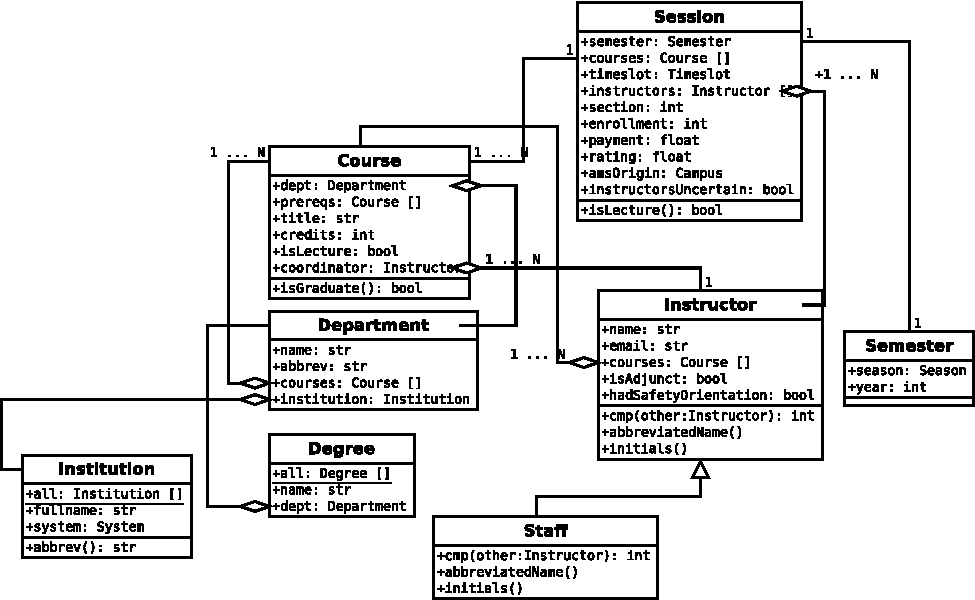
\includegraphics[width=4in]{uml.pdf}
  \end{center}
  \textit{curriculorum} is installed as a Python module and contains
  no institution-specific data (mostly classes).
\end{frame}

\begin{frame}
  \frametitle{Directory Layout}

  An important part of the implementation is getting the directory
  structure right...
  \begin{center}
  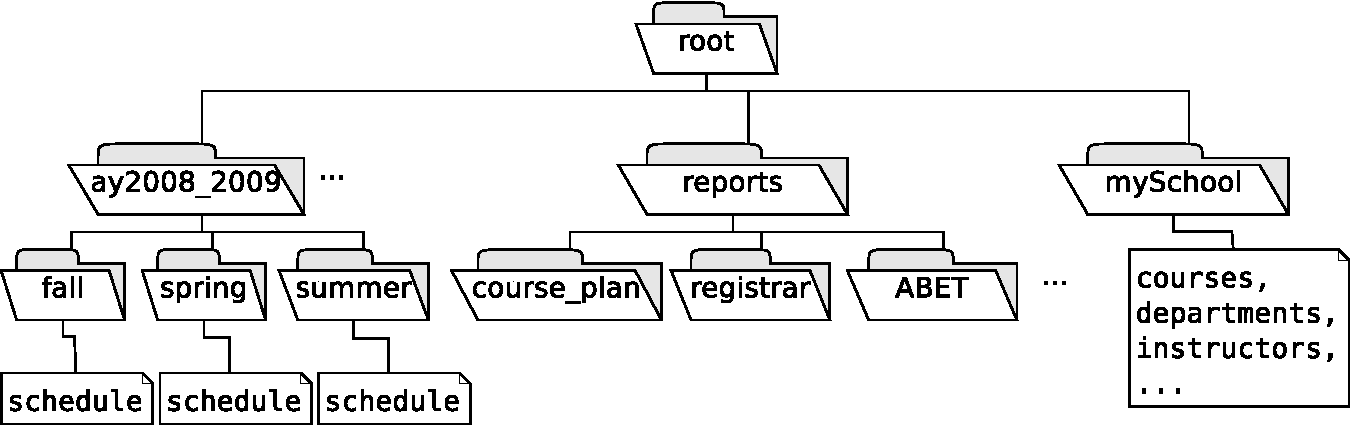
\includegraphics[width=4in]{directories.pdf}
  \end{center}
  \textit{curriculorum} is installed as a Python module and contains
  no institution-specific data (mostly classes).
\end{frame}

\begin{frame}
  \frametitle{Report Generation}

  \begin{itemize}
    \item \textit{curriculorum} generates (\LaTeX) tables.
    \item Tables may be included in \LaTeX~documents (see example).
    \item \textit{curriculorum} can also generate the GraphViz
      ``dot'' format (e.g.) for prerequisite dependency graphs.
  \end{itemize}
\end{frame}

\begin{frame}
  \frametitle{Example: Dependency Graph}

  Here is the dependency tree (DAG, to be precise) \textit{curriculorum}
  automatically derives from prerequisite data:
  \begin{center}
  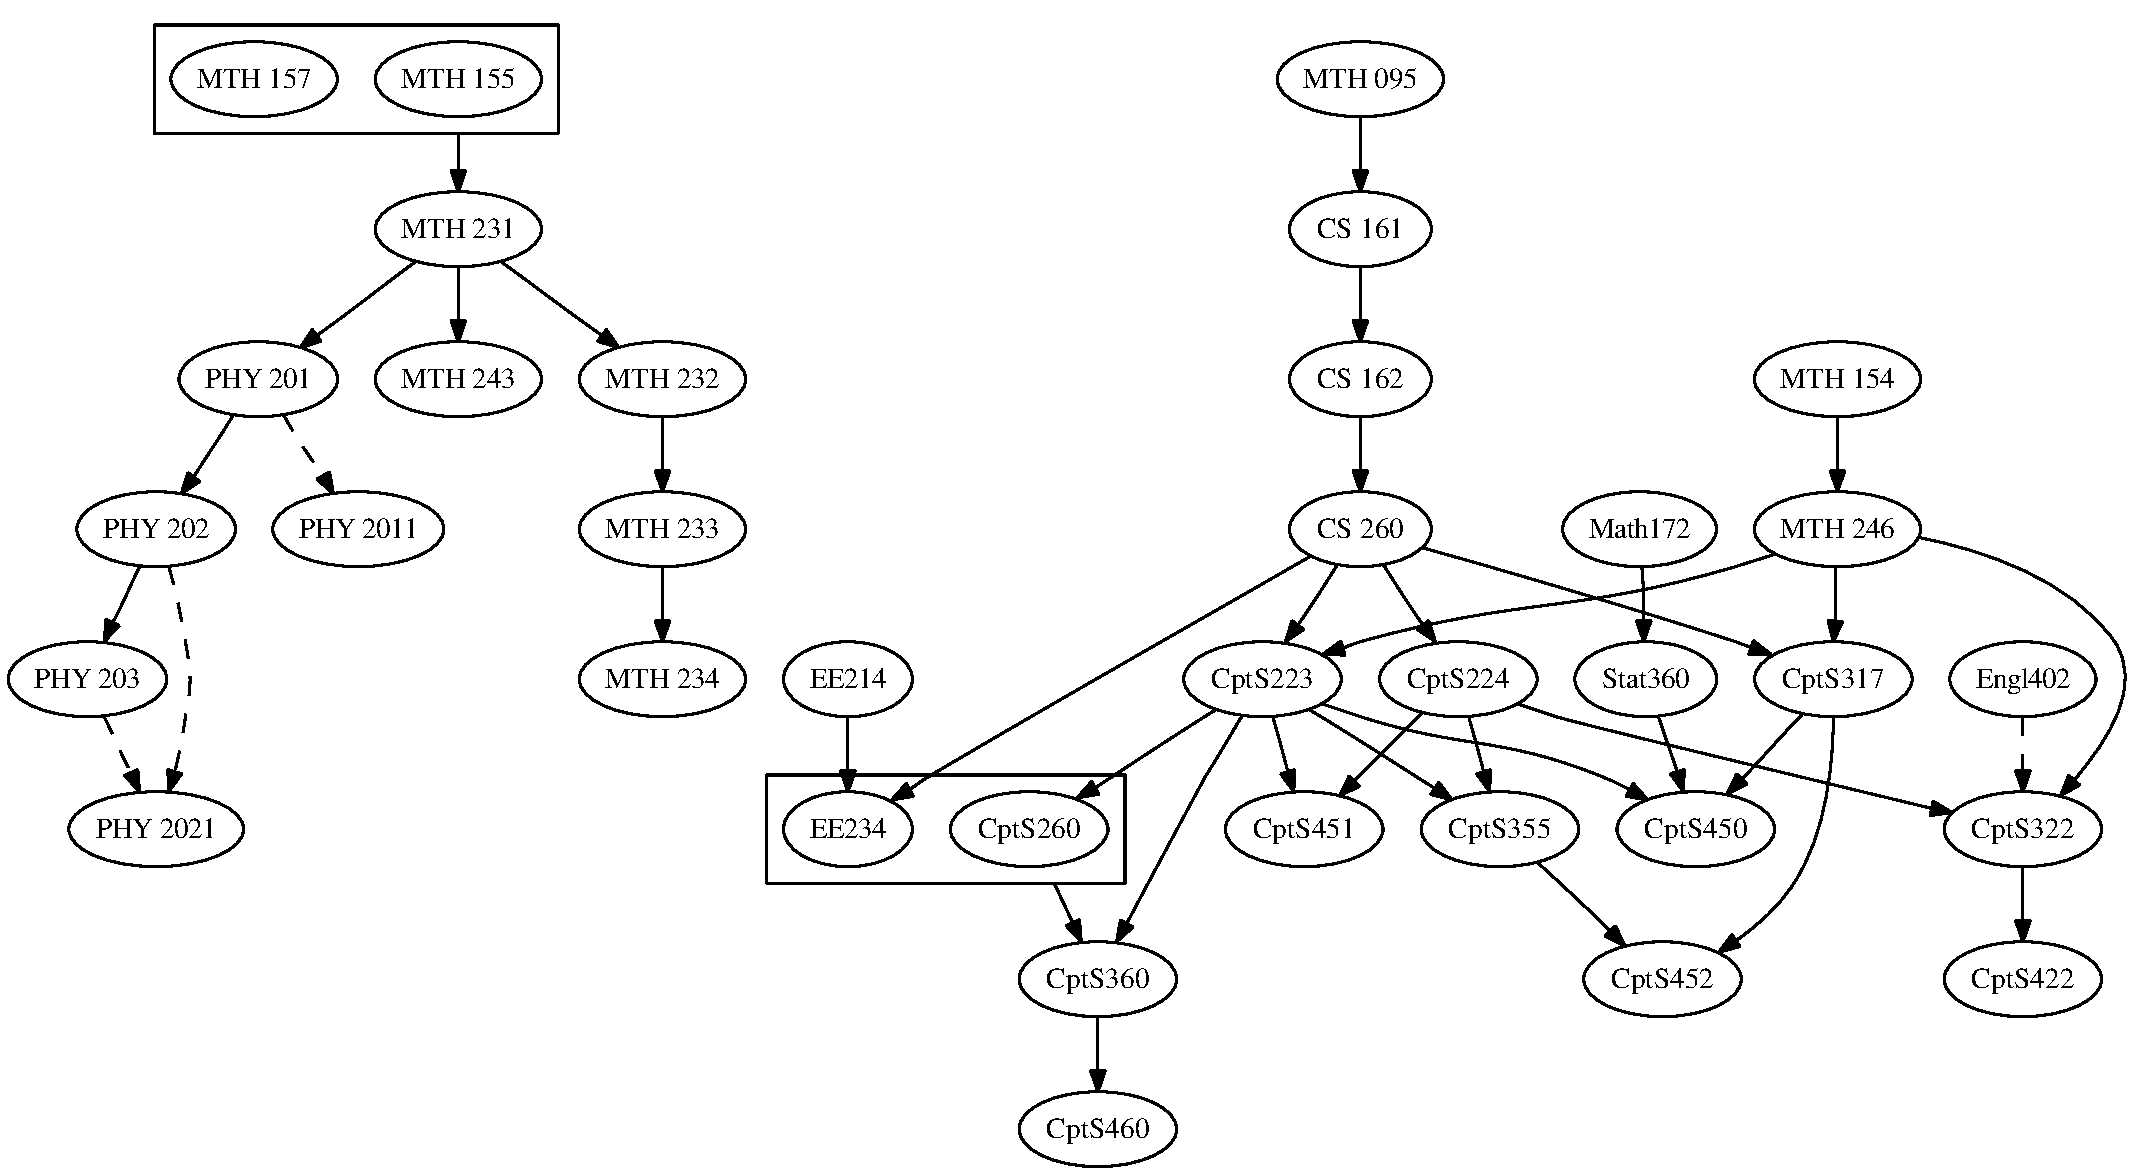
\includegraphics[width=3in]{grph_bscs.pdf}
  \end{center}
  This includes courses at both WSU and Columbia Basin (Community) College.
\end{frame}

\begin{frame}
  \frametitle{A Guided Tour}

  Let's examine some of the files first-hand...
\end{frame}

\section{Conclusions and Future Work}

\begin{frame}
  \frametitle{Conclusions}

  \begin{itemize}
    \item \textit{Curriculorum} has more than justified its
      development time.
    \item It has been in place since 2005, and has adapted to
      curricular changes very well.
    \item Side effect: Developing \textit{curriculorum} has made me a
      better programmer.
  \end{itemize}
\end{frame}

\begin{frame}
  \frametitle{Future Work}

  \begin{itemize}
    \item documenting student specializations (e.g. games, networks,
      software engineering) and showing recommended schedules
    \item additional community college transfer equivalencies
      (i.e. new \texttt{Institution}s)
    \item HTML output (esp. for student perusal)
  \end{itemize}
\end{frame}
\end{comment}
% ---------------------------------------------------------------------------
\begin{comment}



\begin{frame}
  \frametitle{}

\end{frame}

\begin{frame}
  \frametitle{}

  \begin{verbatim}
  \end{verbatim}
\end{frame}

\begin{frame}
  \frametitle{}

  \begin{itemize}
  \item 
  \end{itemize}
\end{frame}


\begin{frame}
  \frametitle{}

  \begin{center}
    \includegraphics[width=\textwidth]{drawings/}
  \end{center}
\end{frame}

\begin{frame}
  \frametitle{}

  \begin{columns}[c]
    \column{0.5\textwidth}
    \column{0.5\textwidth}
  \end{columns}
\end{frame}

\end{comment}
% ---------------------------------------------------------------------------

\end{document}
